\documentclass{beamer}
\usepackage{xmpmulti}
\setbeamertemplate{navigation symbols}{}
\setbeamertemplate{itemize items}[ball]
\usepackage{animate}
\usetheme{default}
\usepackage[style=ieee]{biblatex}
\usecolortheme{seahorse}
\usepackage[]{algorithm2e}
\bibliography{references.bib}
%\setbeamertemplate{navigation symbols}{}
\beamersetuncovermixins{\opaqueness<1>{25}}{\opaqueness<2->{15}}
\begin{document}
\title{Community-based semantic subgroup discovery}
\subtitle{(CBSSD)}
\author{Bla\v{z} \v{S}krlj, An\v{z}e Vavpeti\v{c}, Jan Kralj, Nada Lavra\v{c}}
\date{\today} 

\usebackgroundtemplate{%
  
\includegraphics[width=\paperwidth,height=\paperheight]{images/header}}

\begin{frame}

  {
    \usebackgroundtemplate{
\includegraphics[width=\paperwidth]{images/header.png}}%
    \titlepage
    
  }
  
\end{frame}

\usebackgroundtemplate{%
  
\includegraphics[width=\paperwidth,height=\paperheight]{images/background}}

\begin{frame}\frametitle{Table of contents}\tableofcontents
\end{frame}

\section{General overview} 

\begin{frame}\frametitle{Introduction} 


  \begin{columns}
    \begin{column}{0.5\textwidth}

  \begin{block}{Properties of biological networks}
    \begin{itemize}

    \item Multiple types of nodes and edges $\rightarrow$ heterogenous networks
    \item Possible connections between distinct entities
    \item Large in some sub-domains
    \item Not trivial to interpret
      
    \end{itemize}
  \end{block}
      \end{column}
    \begin{column}{0.5\textwidth}  %%<--- here
      \begin{center}
        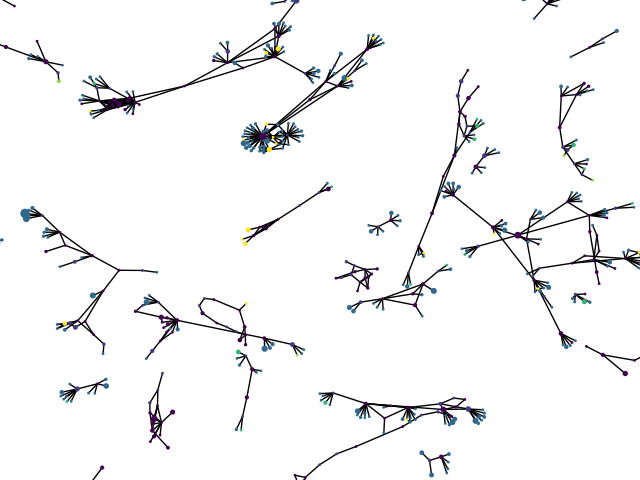
\includegraphics[width=1\textwidth]{images/figure_2}
      \end{center}
    \end{column}
    \end{columns}
  \end{frame}

  \begin{frame}\frametitle{How can an algorithm learn from a complex network?}

    \begin{block}{Network representation}
      Important network features can be encaptured via community detection, graphlets, semantic clustering and other methods..
    \end{block}

    \begin{exampleblock}{Example use}
      Such methodology is used to infer protein-RNA interactions, identify expression patterns, compare protein structures, fuse systems-level data etc.
    \end{exampleblock}
    
  \end{frame}
  
\section{Problem definition} 
  \begin{frame}\frametitle{Problem definition}

    \begin{block}{Term-subset enrichment}
      Let ${t_{1},t_{2},..,t_{n}}$ represent individual terms of interest from the whole term set $\psi $. Identify subsets $\Lambda_{1},\Lambda_{2},..,\Lambda_{n} \subseteq \psi$, which represent interpretable patterns, previously unknown to a human observer.      
    \end{block}

    \begin{exampleblock}{Example situation}

      Let $G_{1},G_{2},..,G_{n}$ be $n$ distinct genes we are interested in. Although individual genes, or the whole group of genes doesn't return any interesting results, we can further explore the subspace of n genes.

    \end{exampleblock}
    \begin{alertblock}{Problem}
      Exploring all possible combinations can be computationally expensive procedure, as there are $\sum_{i=2}^{n}\dfrac{n!}{(n-i)!i!}$ possible options.      
    \end{alertblock}      
  \end{frame}

\section{Proposed approach}
  \begin{frame}\frametitle{Fighting the combinatorial explosion}

    We argue there exists an efficient heuristic-based approach.
      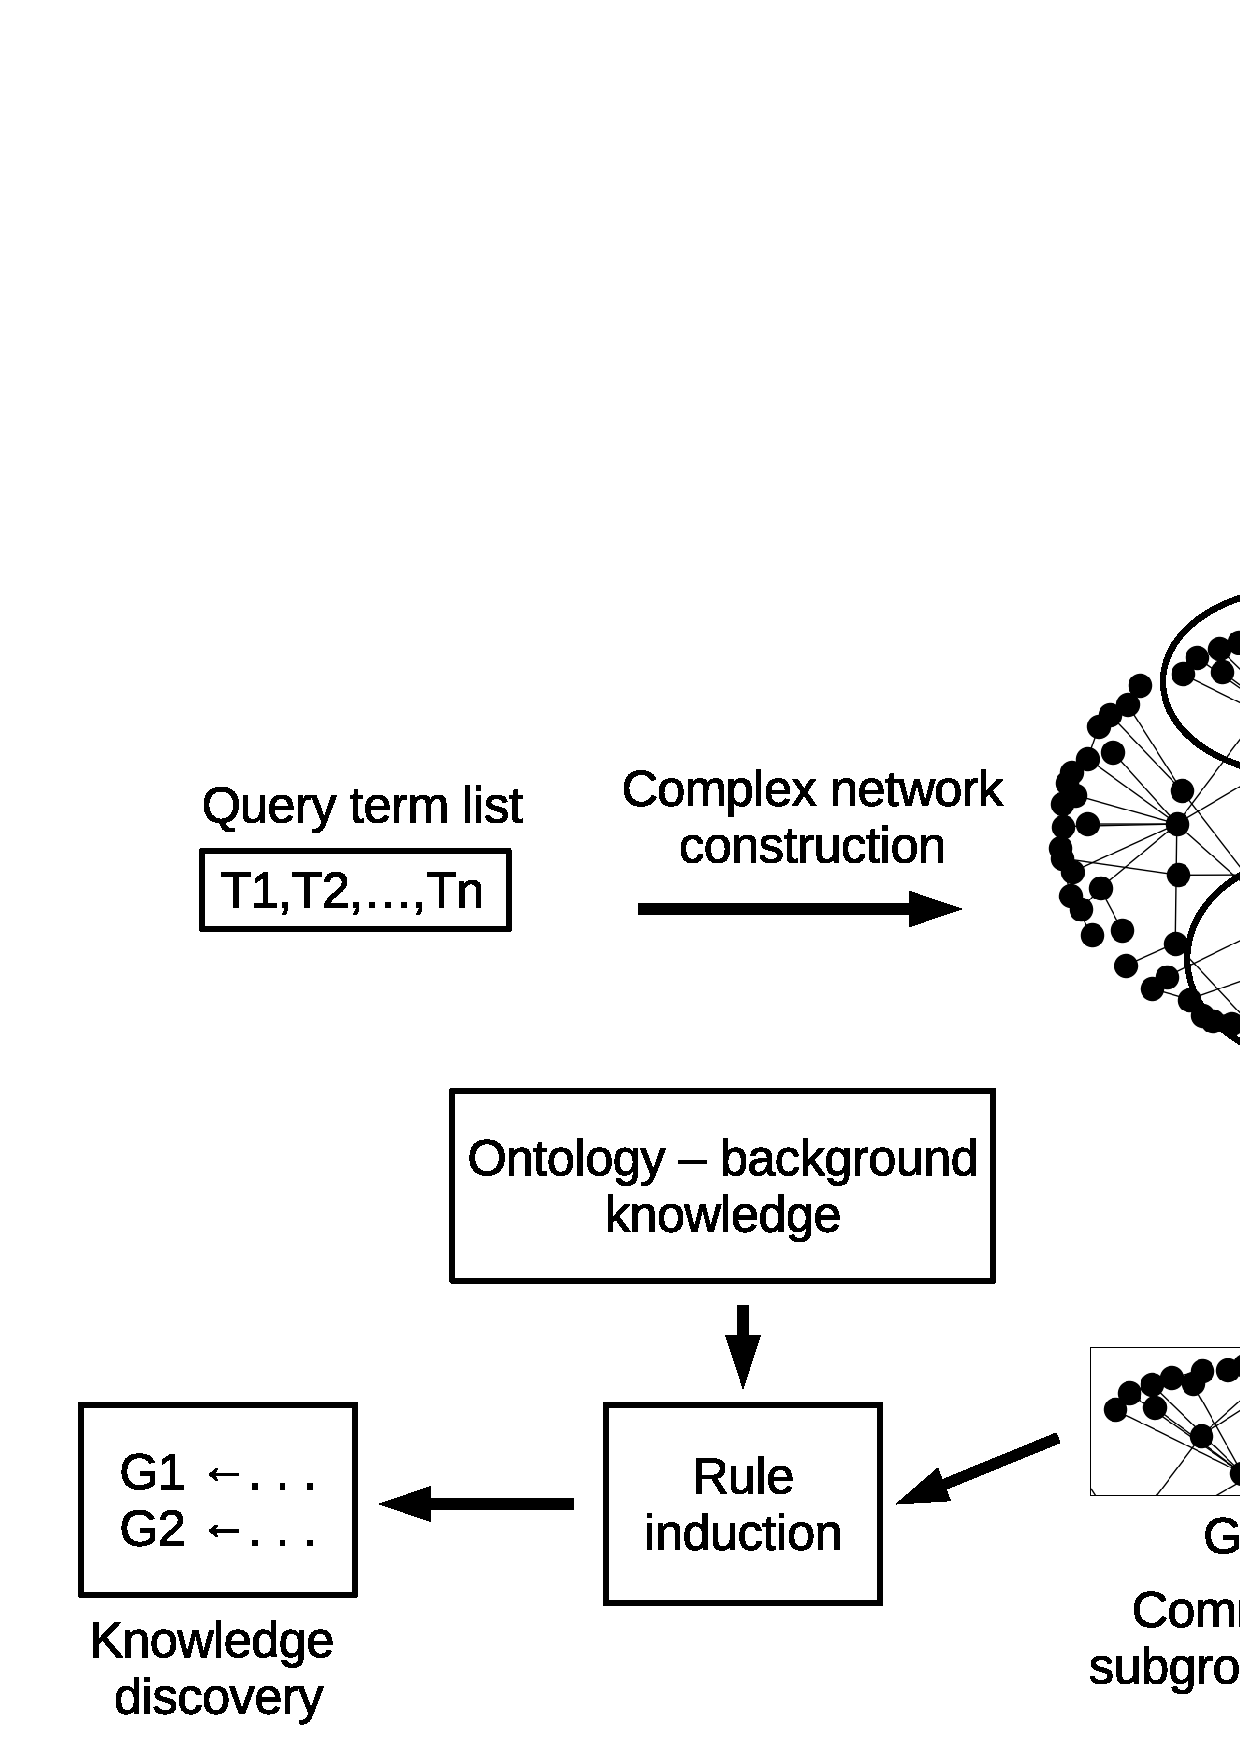
\includegraphics[scale=0.35]{images/workflow2}       
   \end{frame}

  \begin{frame}\frametitle{Fighting the combinatorial explosion - network construction}



  \begin{columns}
    \begin{column}{0.5\textwidth}


      \begin{block}{Basic procedure}
      \begin{itemize}
      \item collect network data on the studied phenomenon
      \item merge the data into a single heterogeneous network
      \item simplify the obtained network, or learn directly from it
      \end{itemize}

      
      \end{block}
      
    \end{column}
    \begin{column}{0.5\textwidth}  %%<--- here
      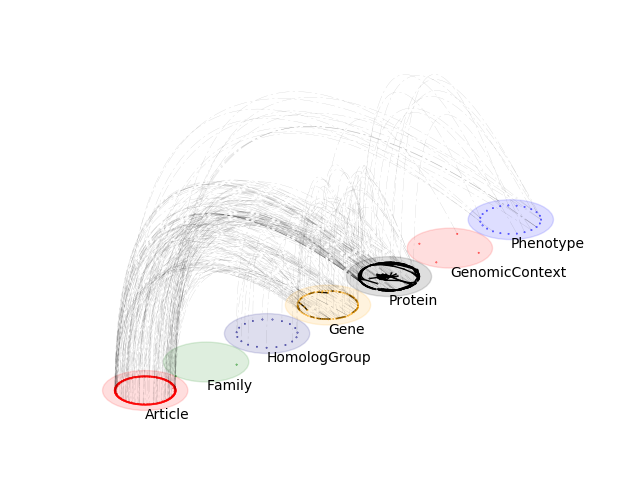
\includegraphics[scale=0.35]{images/figure_1}
    \end{column}
    
  \end{columns}
  
\end{frame}

\begin{frame}\frametitle{Example BioMine network}
%  \transduration<1-4>{2}
%  \multiinclude[<+->][format=png, graphics={width=\textwidth}]{images/simple}
   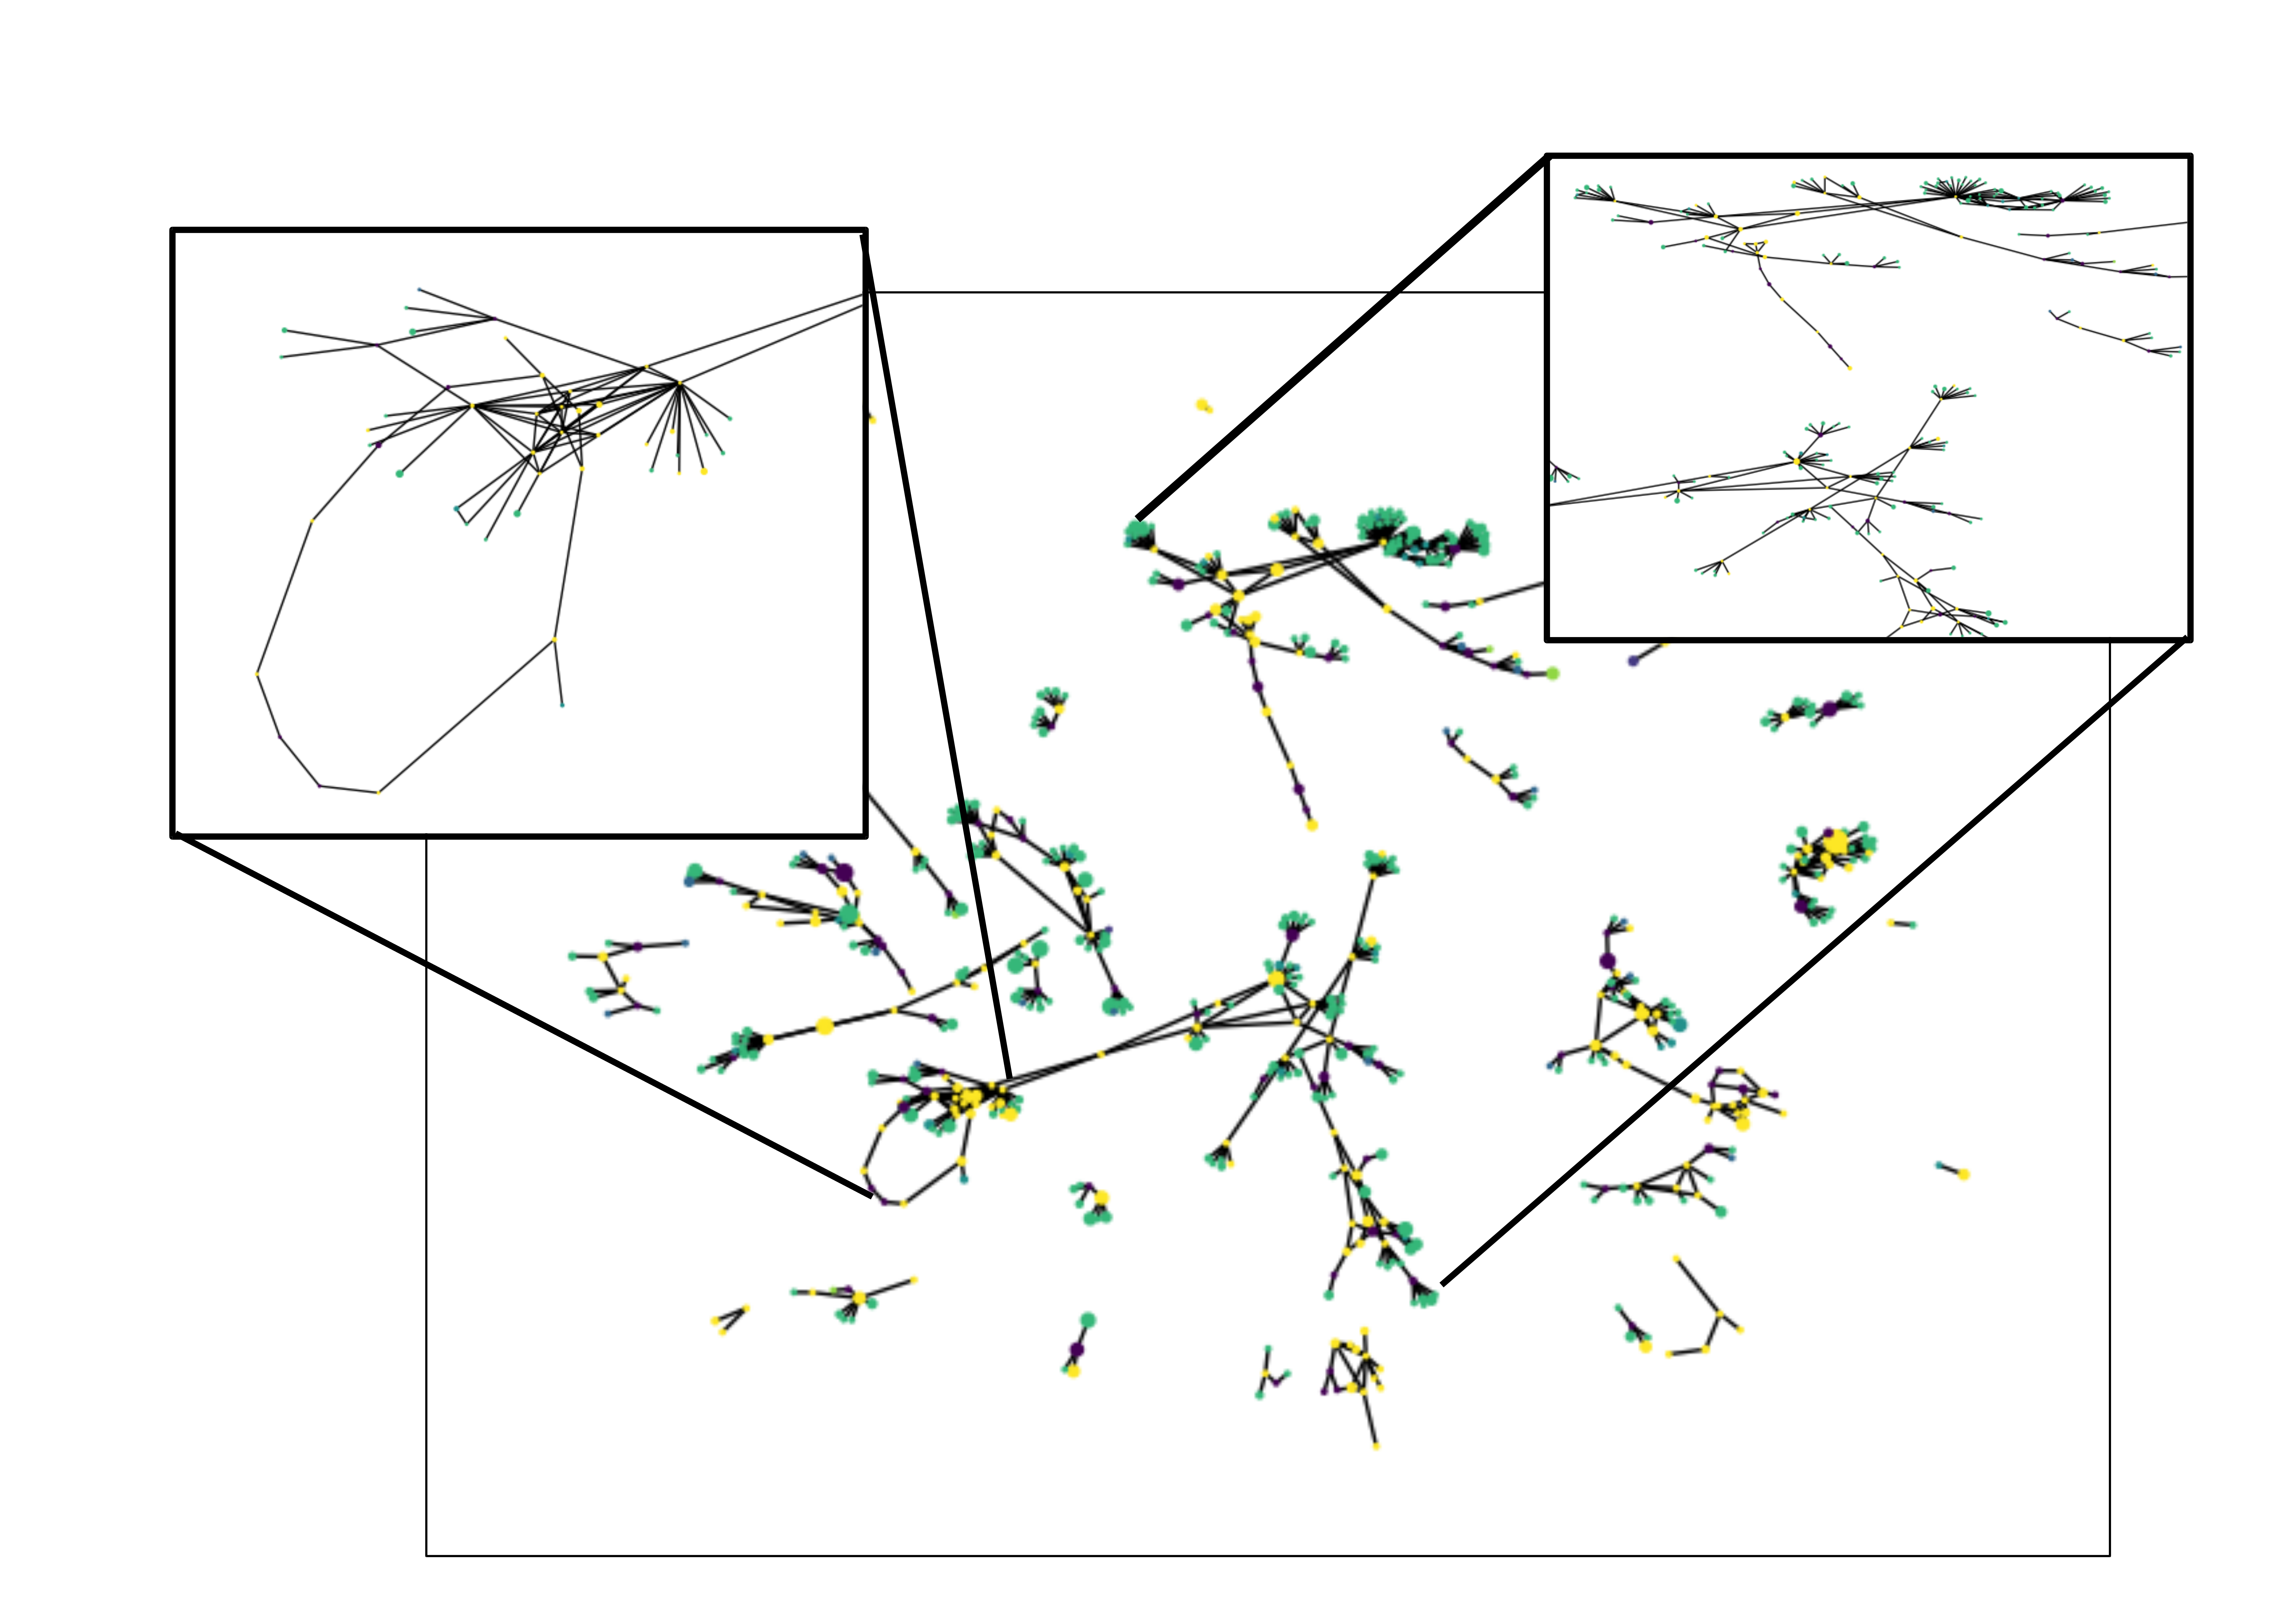
\includegraphics[scale=0.60]{images/collage}
\end{frame}


\begin{frame}\frametitle{Up to 12 layers of interconnected information}  
  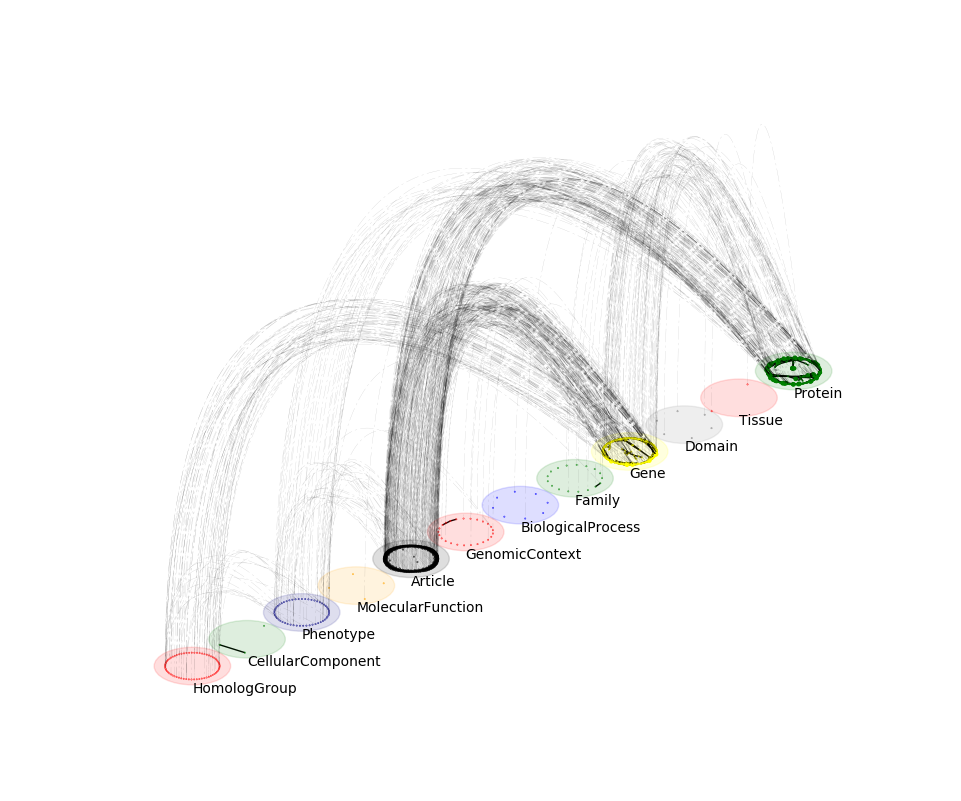
\includegraphics[scale=0.45]{images/SNPmpx}    
\end{frame}

\begin{frame}\frametitle{Subset extraction}

  \begin{block}{Extraction algorithm}
    A multiplex network $ \Psi $ is decomposed into individual communities via the use of $Louvain$ algorithm. Initial term list $\psi $ is then splitted according to community presence, such that initial terms $ t_{1},..,t_{n} $ are assigned to a subset $\zeta_{x,..,y} \in \psi$ $iff$ $\exists t_{x,..,y} \in \Psi_{x,..,y}$.
  \end{block}
  \begin{center}
 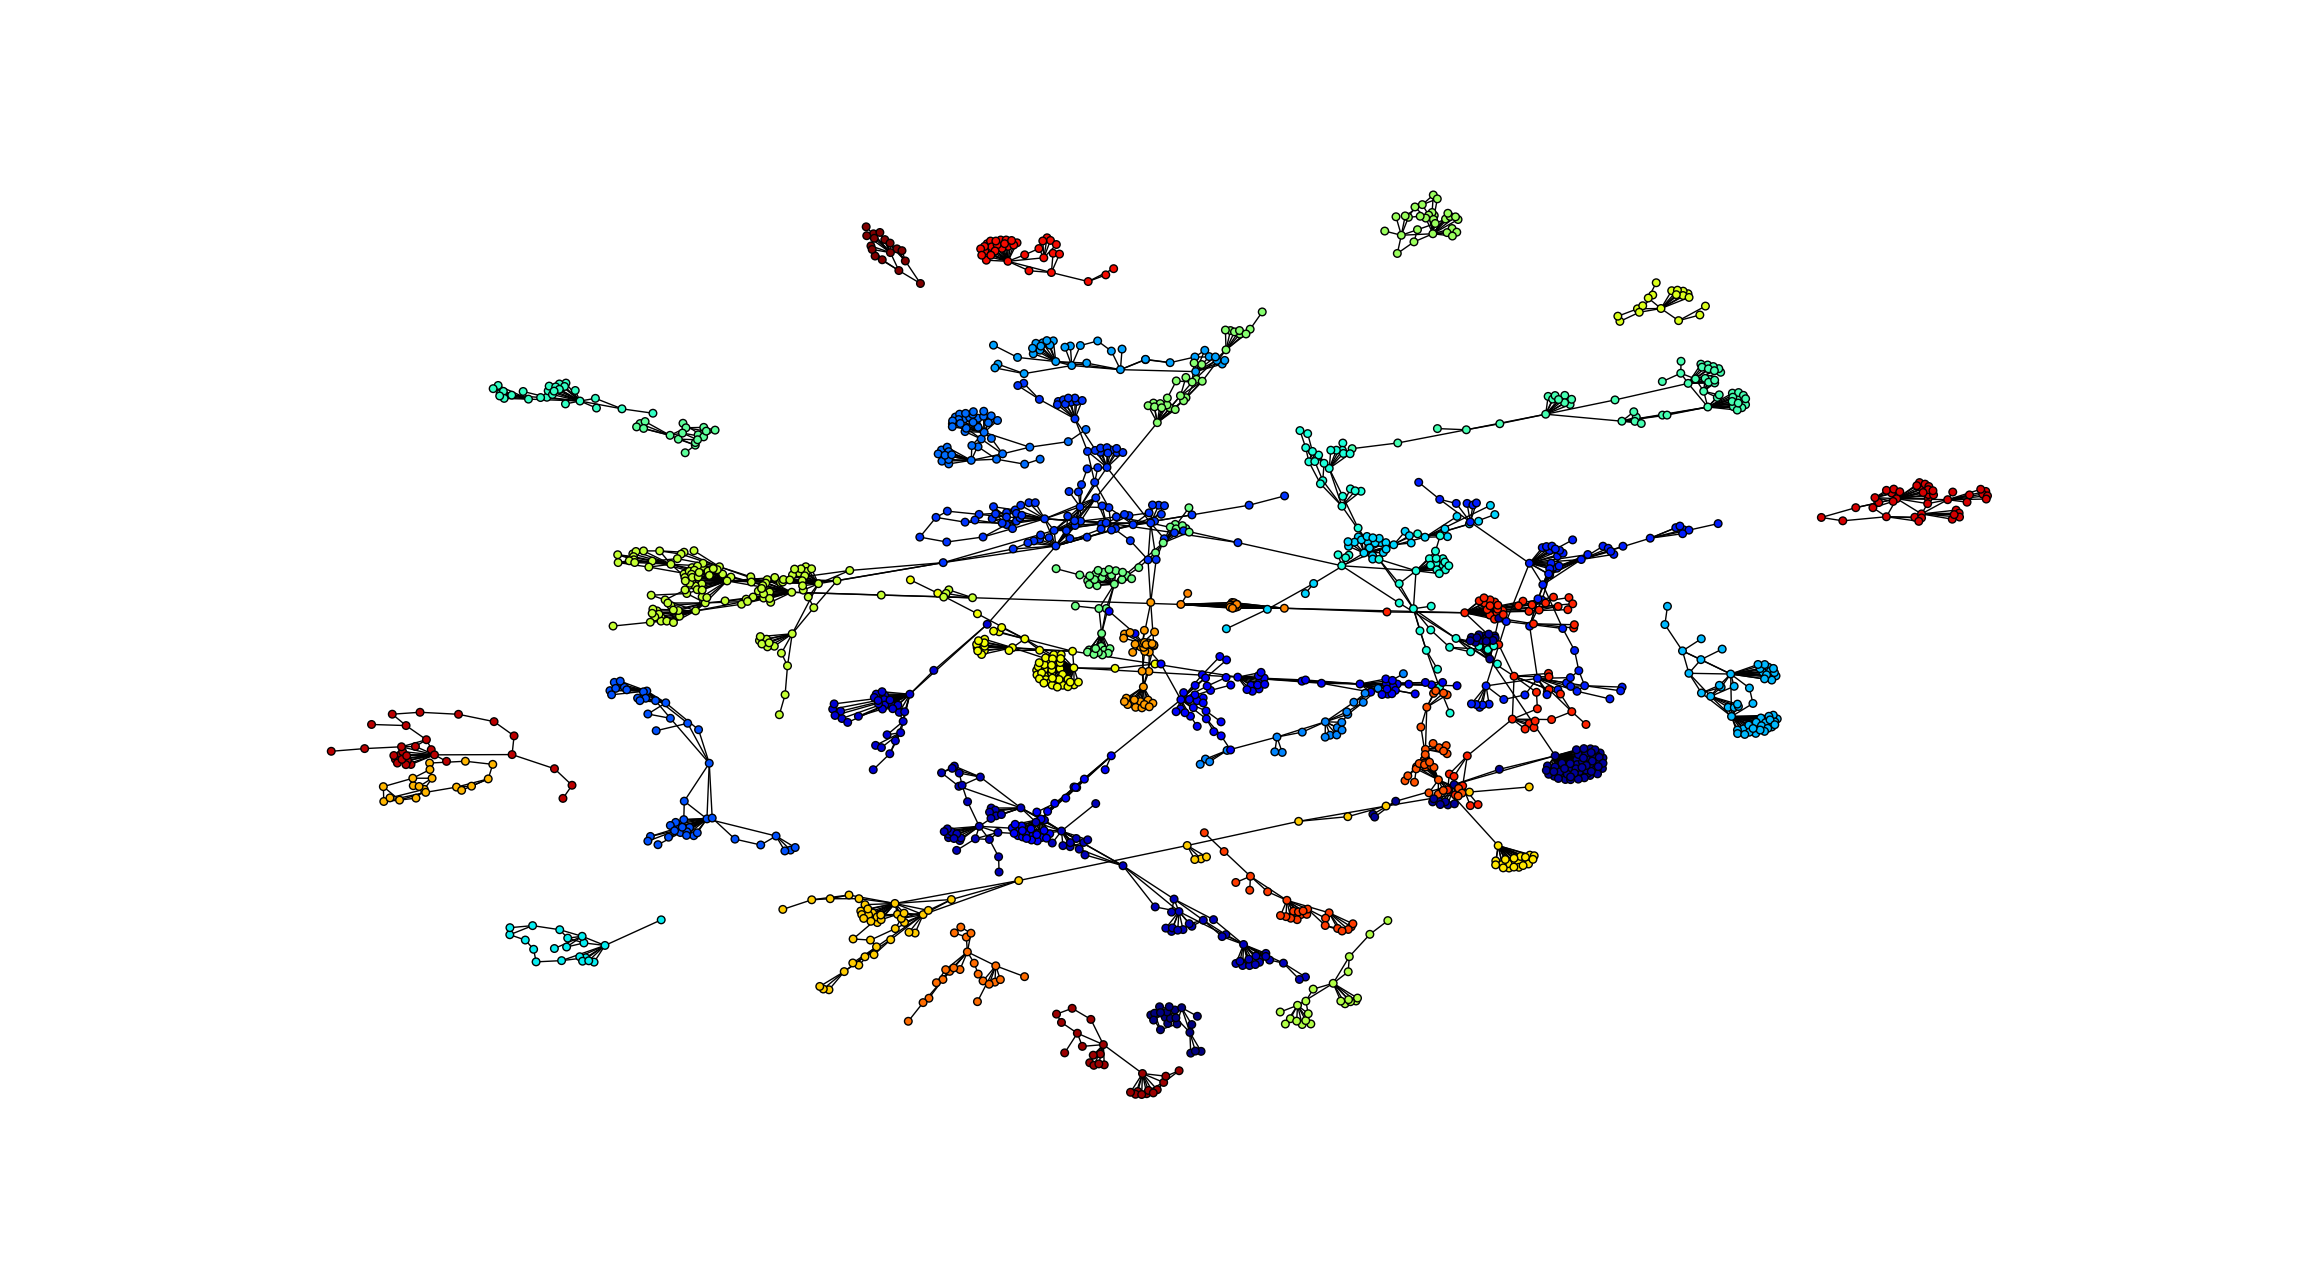
\includegraphics[scale=0.20]{images/biomine_community}
  \end{center}

\end{frame}


\begin{frame}\frametitle{Intermediary result}

  After community detection, the initial term list $\Psi$ is splitted into n smaller subsets $\zeta_{1,..,n}$, which are interpreted as target classes for the semantic rule learning step. The objective function thus becomes:

  \begin{alertblock}{Learning objective}

    Learn a rule set $\Delta_{1,..,n}$  for individual classes $\zeta_{1,..,n}$ using background knowledge ($\Xi$) in form of ontologies, such that the likelihood of individual class $\zeta_{x};x \in \{1,..,n\}$ is maximized.

    \begin{equation}
      \Delta_{\zeta_{1},..,\zeta_{n}} = \underset{i \in R_{1},..,R_{n}}{argmax \Big[P(R_{i}|\Xi) \Big]}
    \end{equation}
    
    \end{alertblock}
  
  \end{frame}

  \begin{frame}\frametitle{Semantic rule learning}

      \begin{columns}
    \begin{column}{0.5\textwidth}

  \begin{block}{Background knowledge representation}
    \begin{itemize}

    \item Individual term sets projected into $\Delta(BK)$ space
    \item Extensive knowledge from $GO,PFAM, KEGG,..$ used
    \item Rules can be generalized according to $BK$
    \item Semi-supervised, multi-class learning problem
      
    \end{itemize}
  \end{block}
      \end{column}
    \begin{column}{0.5\textwidth}  %%<--- here
      \begin{center}
        $R_{1} \rightarrow \bigwedge_{i}GO_{i}; i \in \{GO_{R_{1}}\}$
        $R_{2} \rightarrow \bigwedge_{i}GO_{i}; i \in \{GO_{R_{2}}\}$\\
        $...$\\
        \medskip
        $R_{n} \rightarrow \bigwedge_{i}GO_{i}; i \in \{GO_{R_{n}}\}$
      \end{center}
    \end{column}
    \end{columns}

  \end{frame}
\section{Use case} 
  \begin{frame}\frametitle{Practical example - SNPs}

    \begin{block}{Description}
      SNPs within protein binding sites previously identified term set $\psi$ indicates association with DNA-related processes, cancer development and membrane mechanisms. We were interested, whether there exist more detailed, yet generalized properties of the studied phenomenon.
    \end{block}
  \end{frame}


  \begin{frame}\frametitle{Practical example - SNPs (2)}

    %% overview in numbers!

  \end{frame}

\end{document}